\documentclass[12pt,a5paper]{article}
\usepackage{rmpackages}																% usual packages
\usepackage{rmtemplate}																% graphic charter
\usepackage{rmexocptce}																% for DS with cptce eval
\cfoot{} 													% if no page number is needed
%\renewcommand\arraystretch{1.5}		% stretch table line height

\begin{document}

\newgeometry{left=1.5cm,right=1.5cm,top=2cm}
\thispagestyle{empty}

\setcounter{section}{2}

\section{Perception d'un son}

Pour qu'un son soit \textbf{audible}, sa fréquence doit être comprise entre \unit{20}{Hz} et \unit{20}{kHz}.
\begin{center}
\begin{tikzpicture}
\draw [->, > = stealth, gray_f, line width=2] (0,0) -- (10,0) ;
\draw [gray_f] (3,0) node{$|$} node[below]{\unit{20}{Hz}};
\draw [gray_f] (7,0) node{$|$} node[below]{\unit{20}{kHz}};
\draw [gray_f] (10,0) node[below right]{$f$};
\draw (1.5,0) node[above]{Infrasons};
\draw (5,0) node[above]{\textbf{Sons audibles}};
\draw (8.5,0) node[above]{Ultrasons};
\end{tikzpicture}
\end{center}

\subsection{Hauteur et timbre}

La \textbf{hauteur} d'un son dépend de sa fréquence :
\begin{itemize}
\item[•] plus un son est \textbf{aigu}, plus sa fréquence est élevée ;
\item[•] plus un son est \textbf{grave}, plus sa fréquence est basse.
\end{itemize}

Le \textbf{timbre} d'un son est lié à la forme du signal sonore.

\noindent
\textit{
Exemple : Les deux sons représentés ci-dessous ont la même hauteur mais des timbres différents.
}
\begin{center}
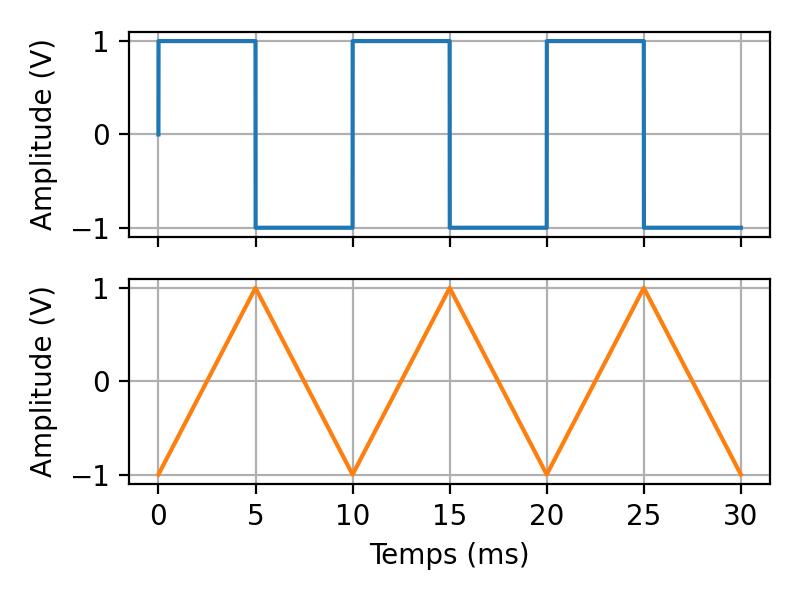
\includegraphics[scale=0.75]{images/hauteur_timbre.png}
\end{center}

\subsection{Niveau d'intensité sonore}

Le \textbf{niveau d'intensité sonore} s'exprime en décibel (dB).
Plus l'intensité sonore est grande, plus le niveau d'intensité sonore est élevé.

\end{document}